\documentclass{beamer}
\usepackage{beamerthemeshadow}
\usepackage[latin1]{inputenc}
\usepackage[english]{babel}
\usepackage{amsmath}
\usepackage{amssymb}
\usepackage{color}
\usepackage{lscape}
\usepackage{alltt}
\usepackage{array}
\usepackage{color}
\usepackage{listings}
\usepackage{graphicx}
\usepackage{csquotes}
\usepackage{caption}
\usepackage{subcaption}
\usepackage{soul}

\setbeamertemplate{footline}[frame number]
\graphicspath{ {images/} }

\begin{document}

% title page
\title{ HAEOLUS - green hydrogen produced in Berlev\r{a}g, Norway}
\author{Nicolas Holland}


\frame{\titlepage} 

\frame{\frametitle{Overview}
\begin{enumerate}
\item Location
\item Companies involved
\item About the wind park
\item About the hydrogen plant
\item Plans for expansion
\item Additional challenges
\end{enumerate}
}


\frame{\frametitle{Location}
Both the wind park and hydrogen plant are located near to Berlev\r{a}g, Norway, well within the artic circle. Winds are strong there and the city which is a fishing hub has a harbor that can service ships.\\
\ \\
\begin{minipage}{.5\textwidth}
\centering
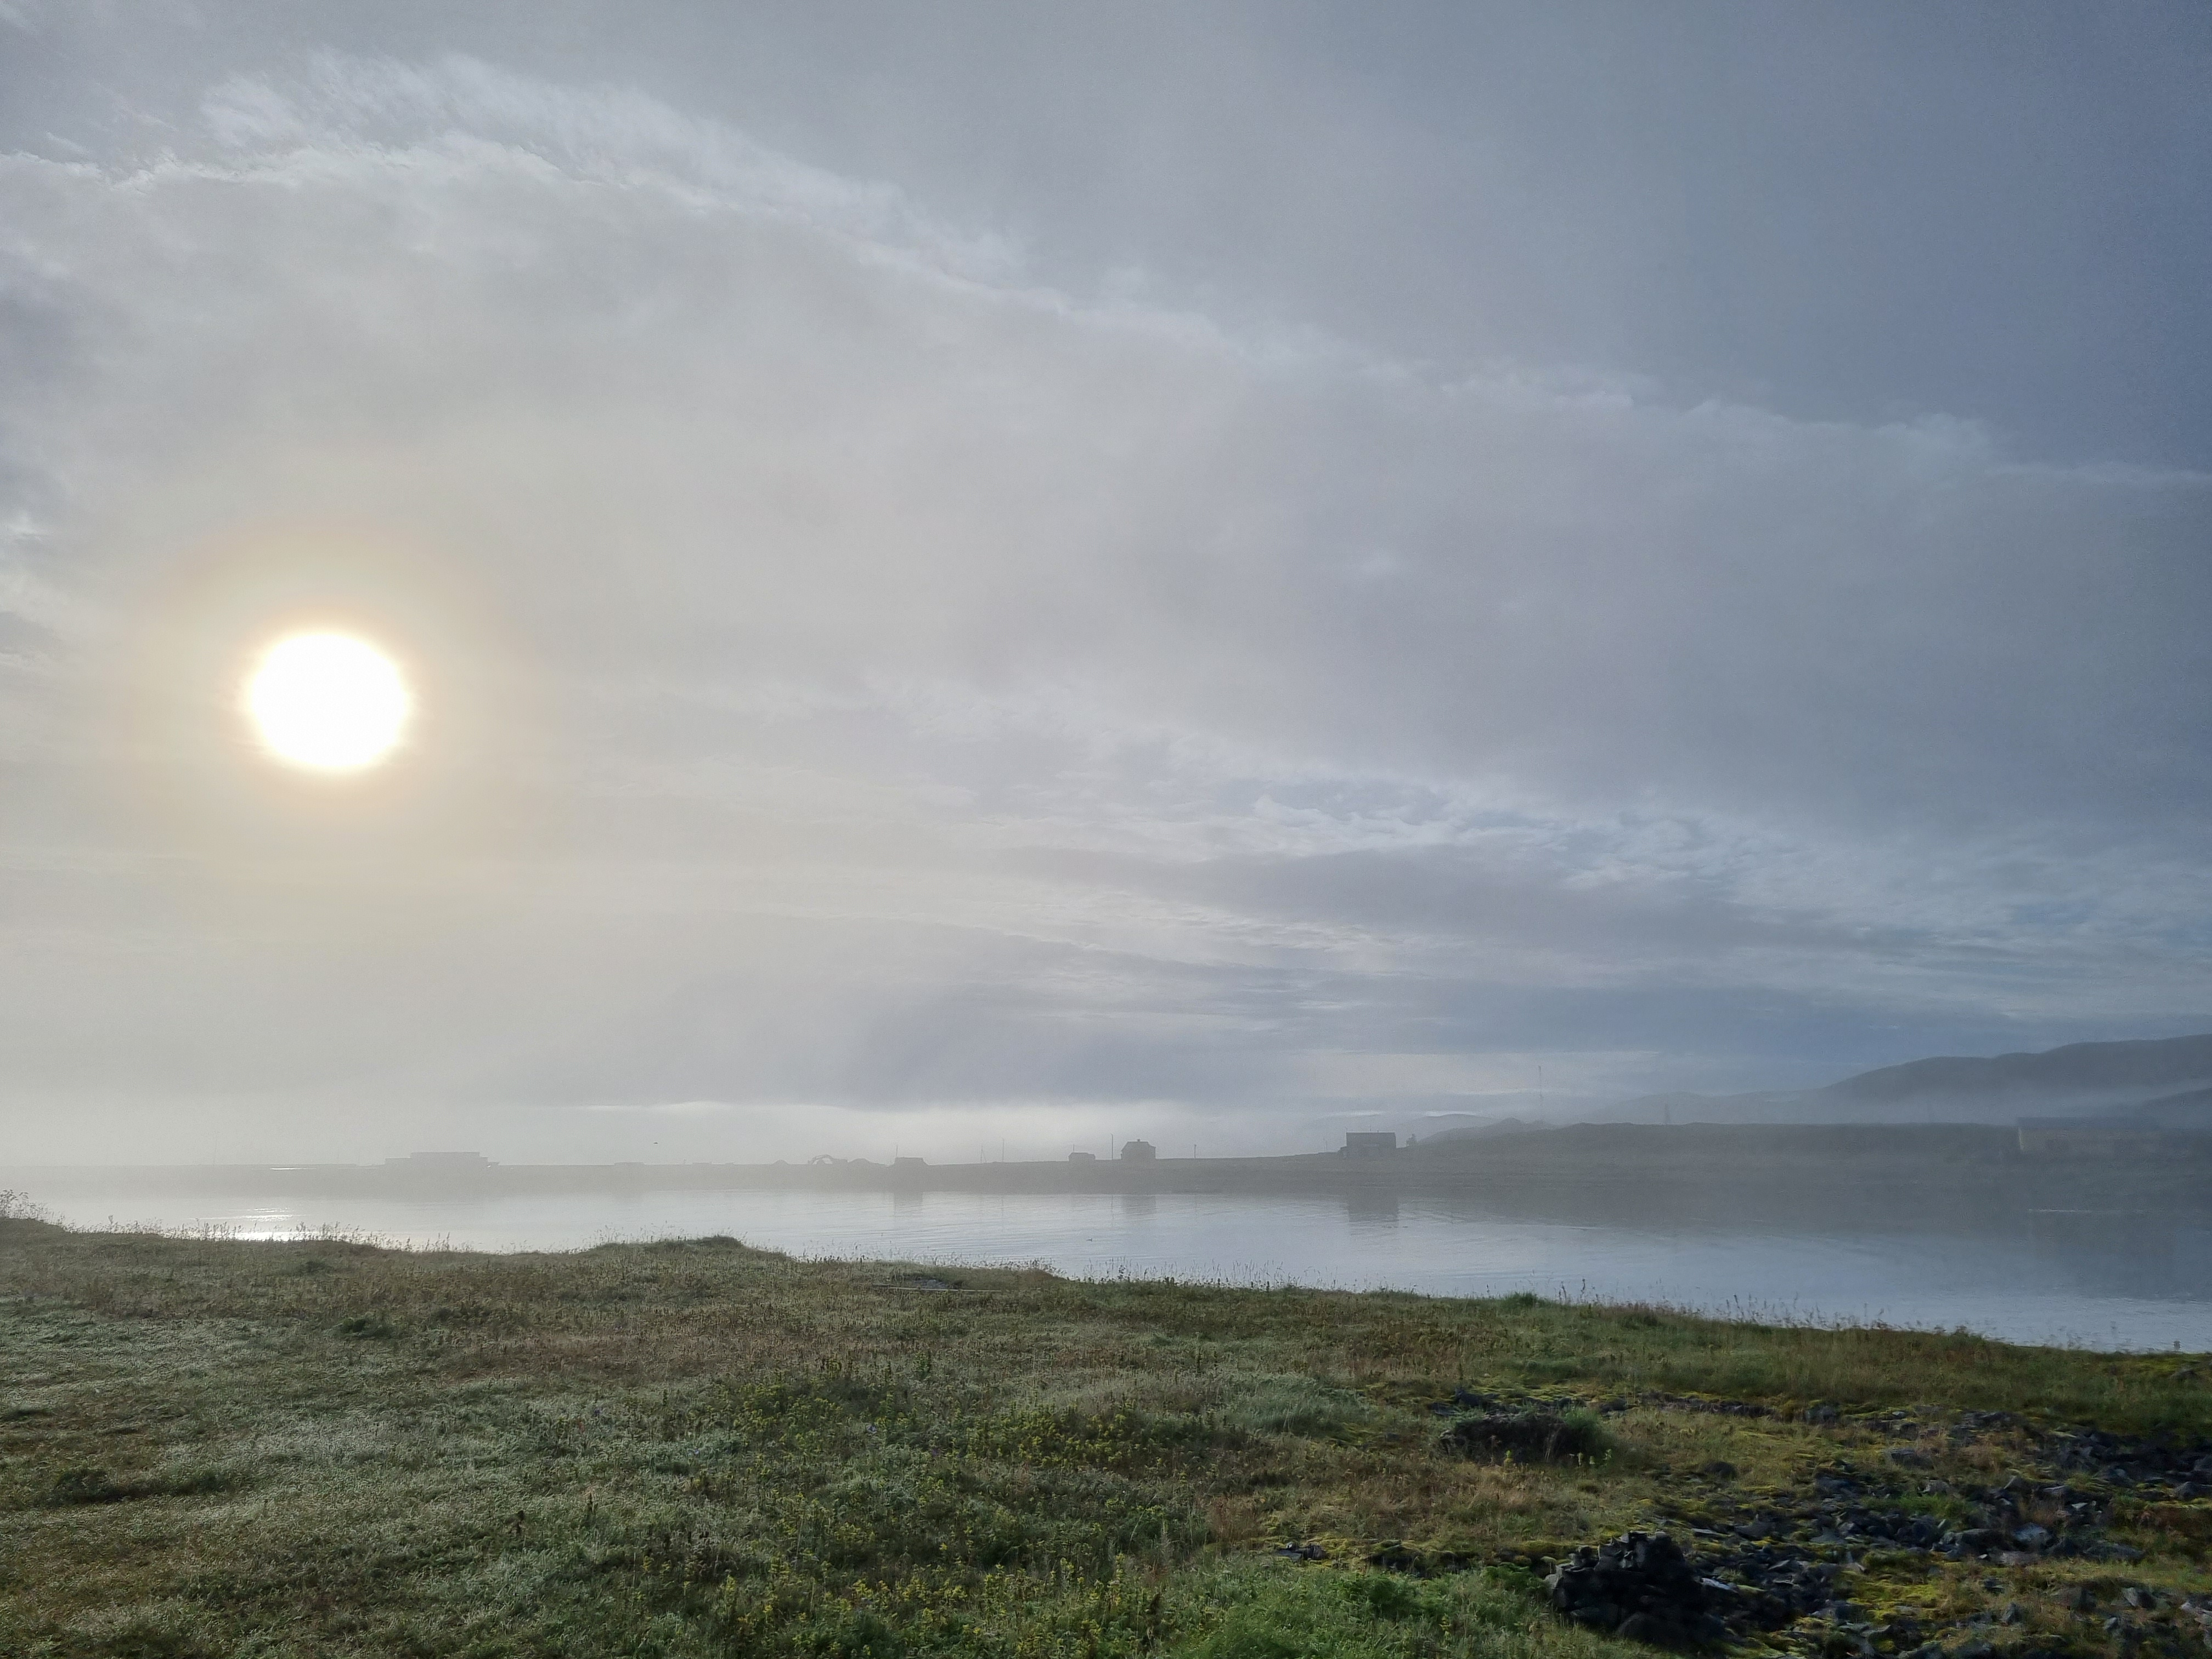
\includegraphics[scale=0.04]{i1}
\end{minipage}%
\begin{minipage}{.5\textwidth}
\centering
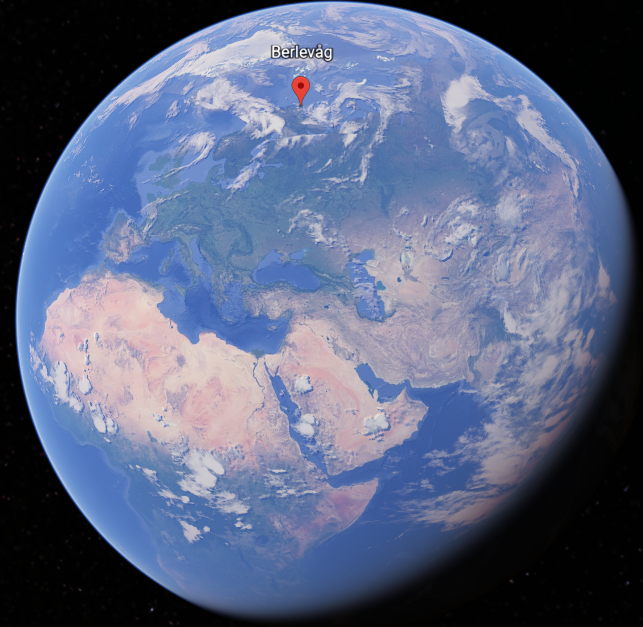
\includegraphics[scale=0.25]{i2}
\end{minipage}%
}


\frame{\frametitle{Companies involved}
Here are some of the companies that are directly involved
\begin{enumerate}
\item Varanger Kraft - Power company, municipal owned
\item Cummins - Electrolyzers
\item Hydrogenics - Hydrogen and fuel cells (aquired by Cummins)
\end{enumerate}
indirectly involved companies include Siemens, who built and maintain the wind turbines, as well as companies that did the yield assessment for the wind park or that are involved in the investment.
}

\frame{\frametitle{About the wind park}
\begin{minipage}{.5\textwidth}
\centering
\begin{enumerate}
\item Wind park in east Finnmark with ~45MW capacity
\item A single turbine has about ~3MW capacity
\item Finnmark is an energy rich region with hydro power\\ and lots of arctic wind
\end{enumerate}
\end{minipage}%
\begin{minipage}{.5\textwidth}
\centering
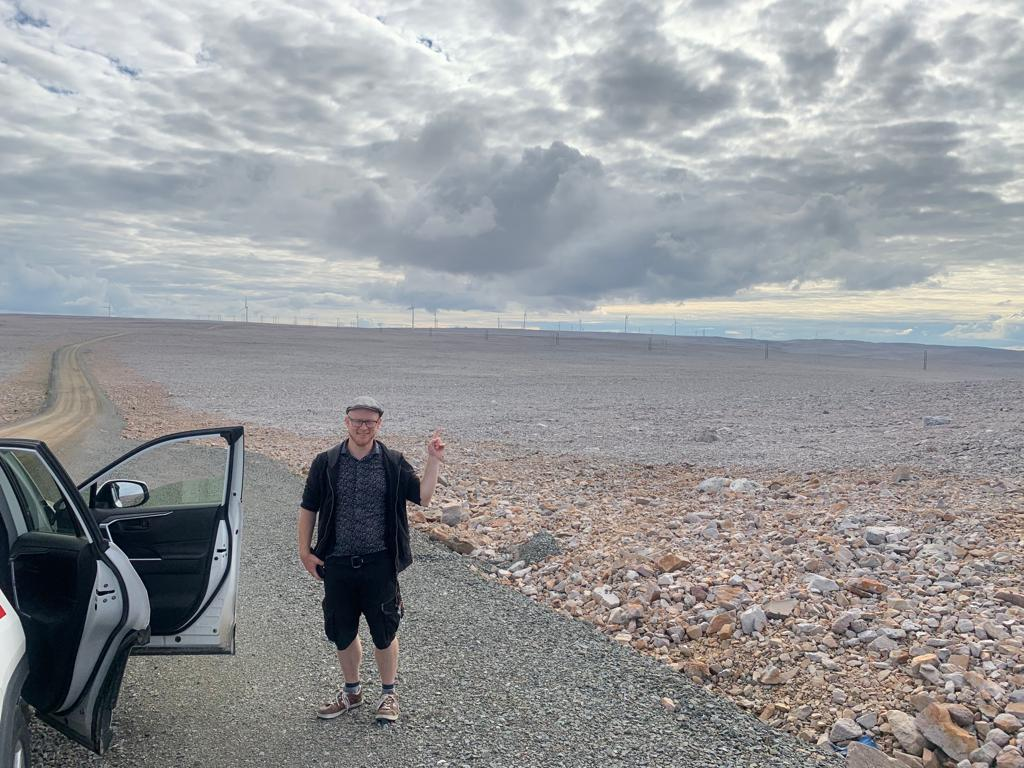
\includegraphics[scale=0.17]{i3}
\end{minipage}%
}

\frame{\frametitle{About the wind park}
\begin{minipage}{.5\textwidth}
\begin{enumerate}
\item Due to political reasons, concessions for new plants are rare and valuable
\item There are plans to expand the park to ~200MW capacity
\item The Norwegian power grid\\ is not able to transport that energy to the south; therefore it needs to be utilized up in the north
\end{enumerate}
\end{minipage}%
\begin{minipage}{.5\textwidth}
\centering
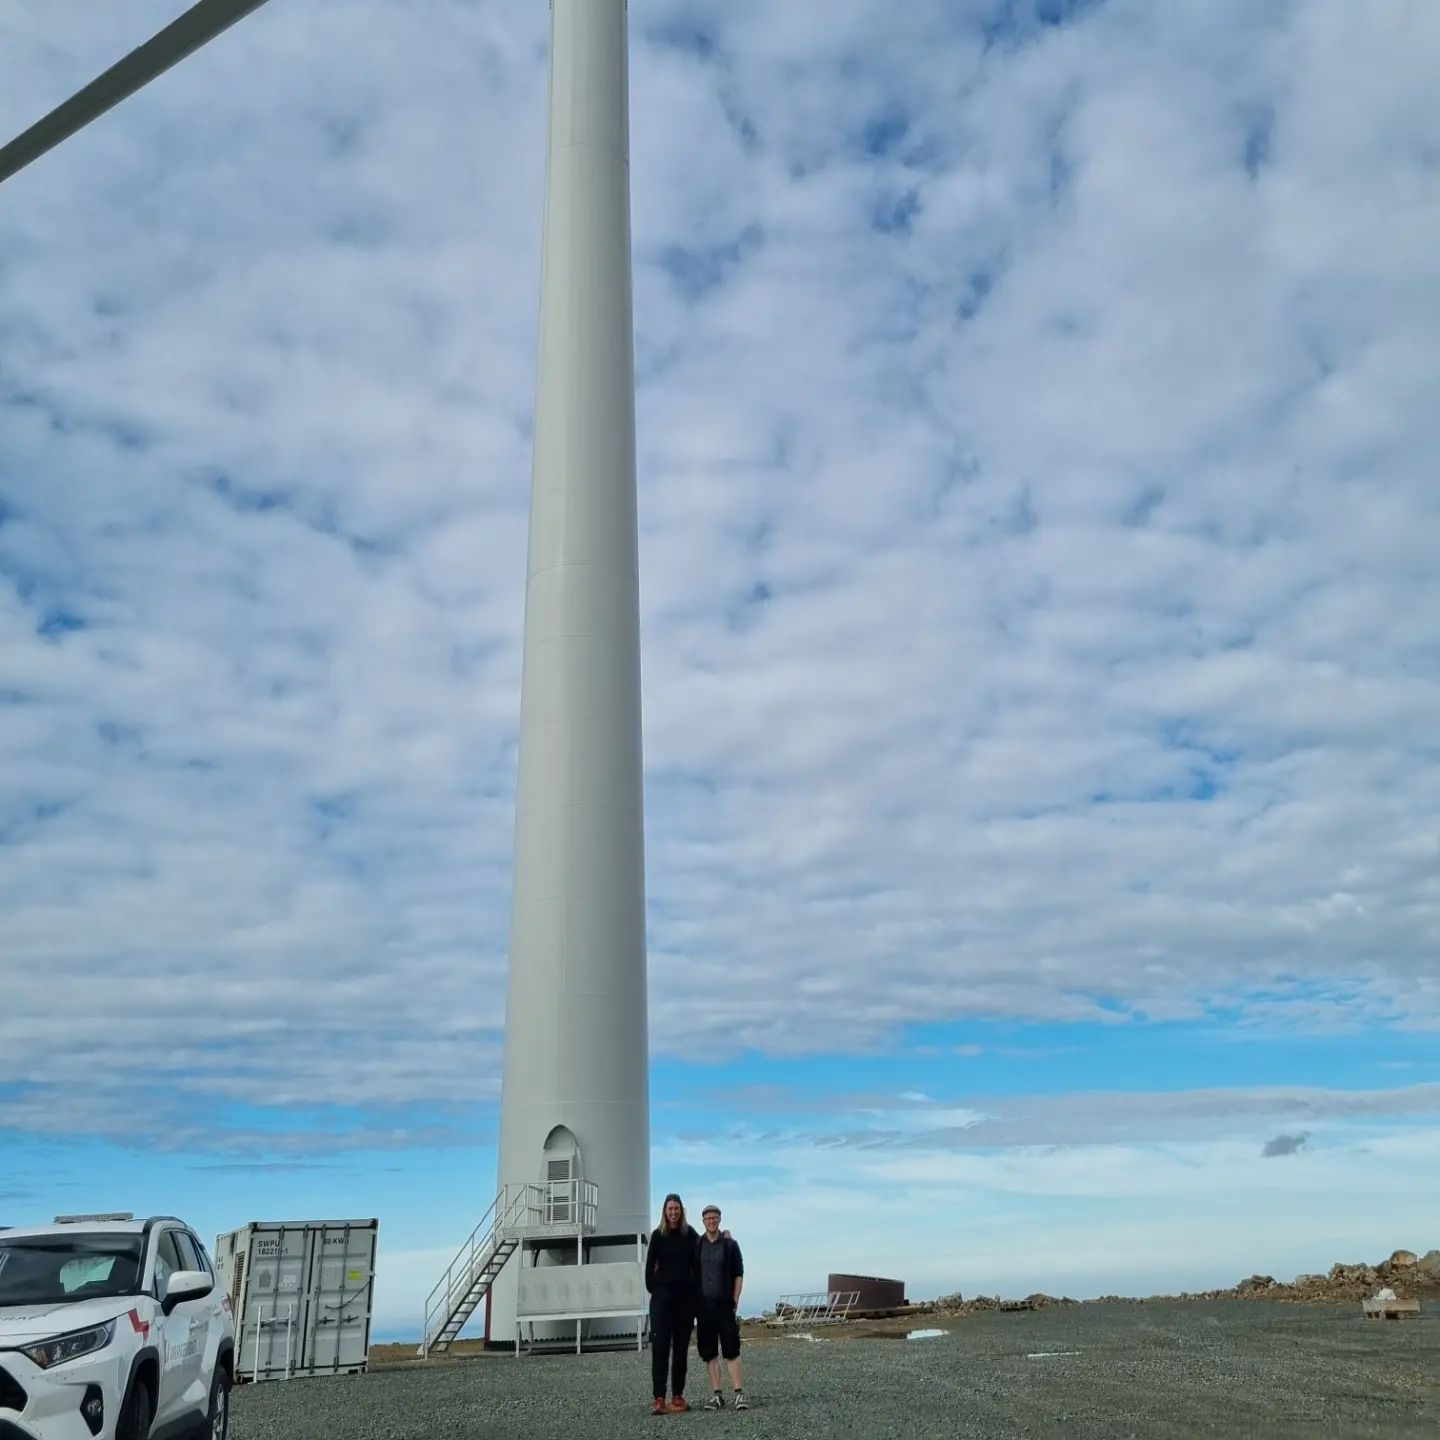
\includegraphics[scale=0.12]{i4}
\end{minipage}%
}

\frame{\frametitle{About the hydrogen plant}
\begin{minipage}{.5\textwidth}
\centering
\begin{enumerate}
\item Haeolus project funded by European Union
\item Production of green hydrogen from artic wind power
\item Research there includes control algorithms to optimize the utilization of available wind power
\end{enumerate}
\end{minipage}%
\begin{minipage}{.5\textwidth}
\centering
\includegraphics[scale=0.04]{i5}
\end{minipage}%
}


\frame{\frametitle{About the hydrogen plant}
\begin{minipage}{.5\textwidth}
\centering
\begin{enumerate}
\item Three containers in the plant: Transformers, electrolyzers and fuel cell
\item Power is generated primarily at the wind park
\item Electrolyzers have 2.5MW capacity
\end{enumerate}
\end{minipage}%
\begin{minipage}{.5\textwidth}
\centering
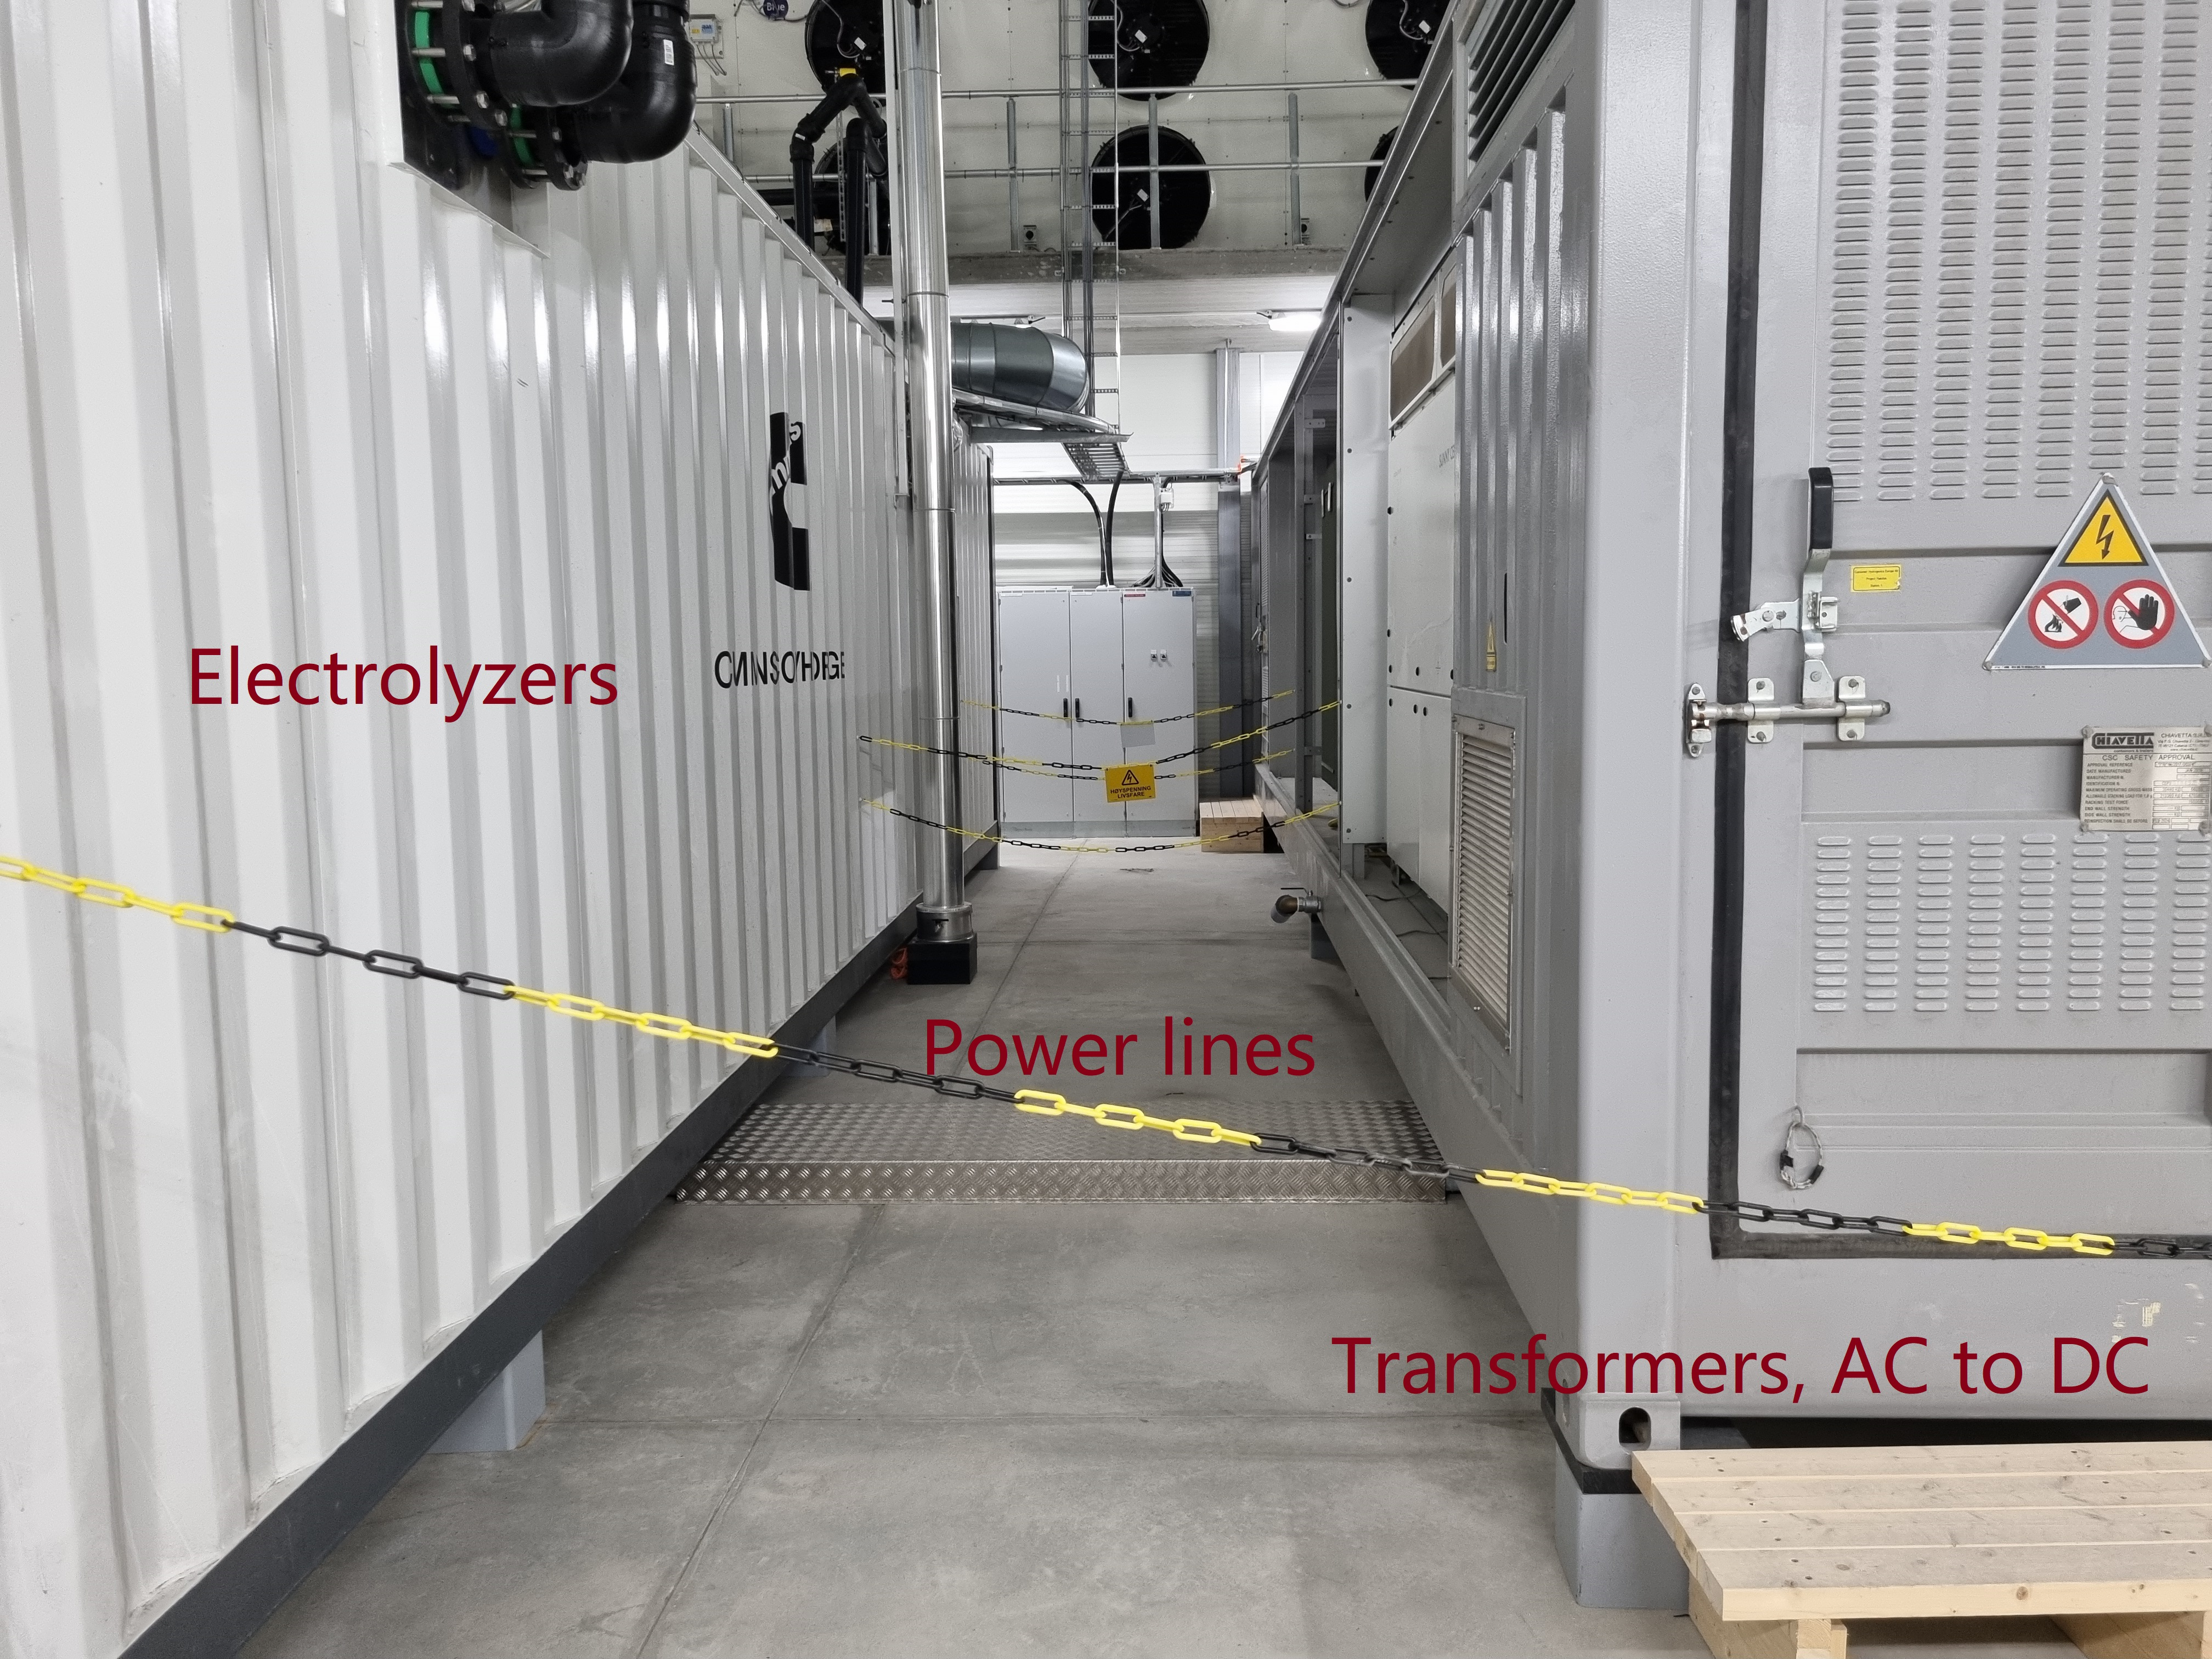
\includegraphics[scale=0.04]{container1}
\end{minipage}%
}

\frame{\frametitle{About the hydrogen plant}
\begin{minipage}{.5\textwidth}
\centering
\begin{enumerate}
\item Fuel cell is rather small to avoid having the plant be regulated as a power producer
\item There are infrared cameras and gas sensors to detect hydrogen leaks
\item Electrolyzers are operated mostly remotly with the occasional need for on-site maintenance
\end{enumerate}
\end{minipage}%
\begin{minipage}{.5\textwidth}
\centering
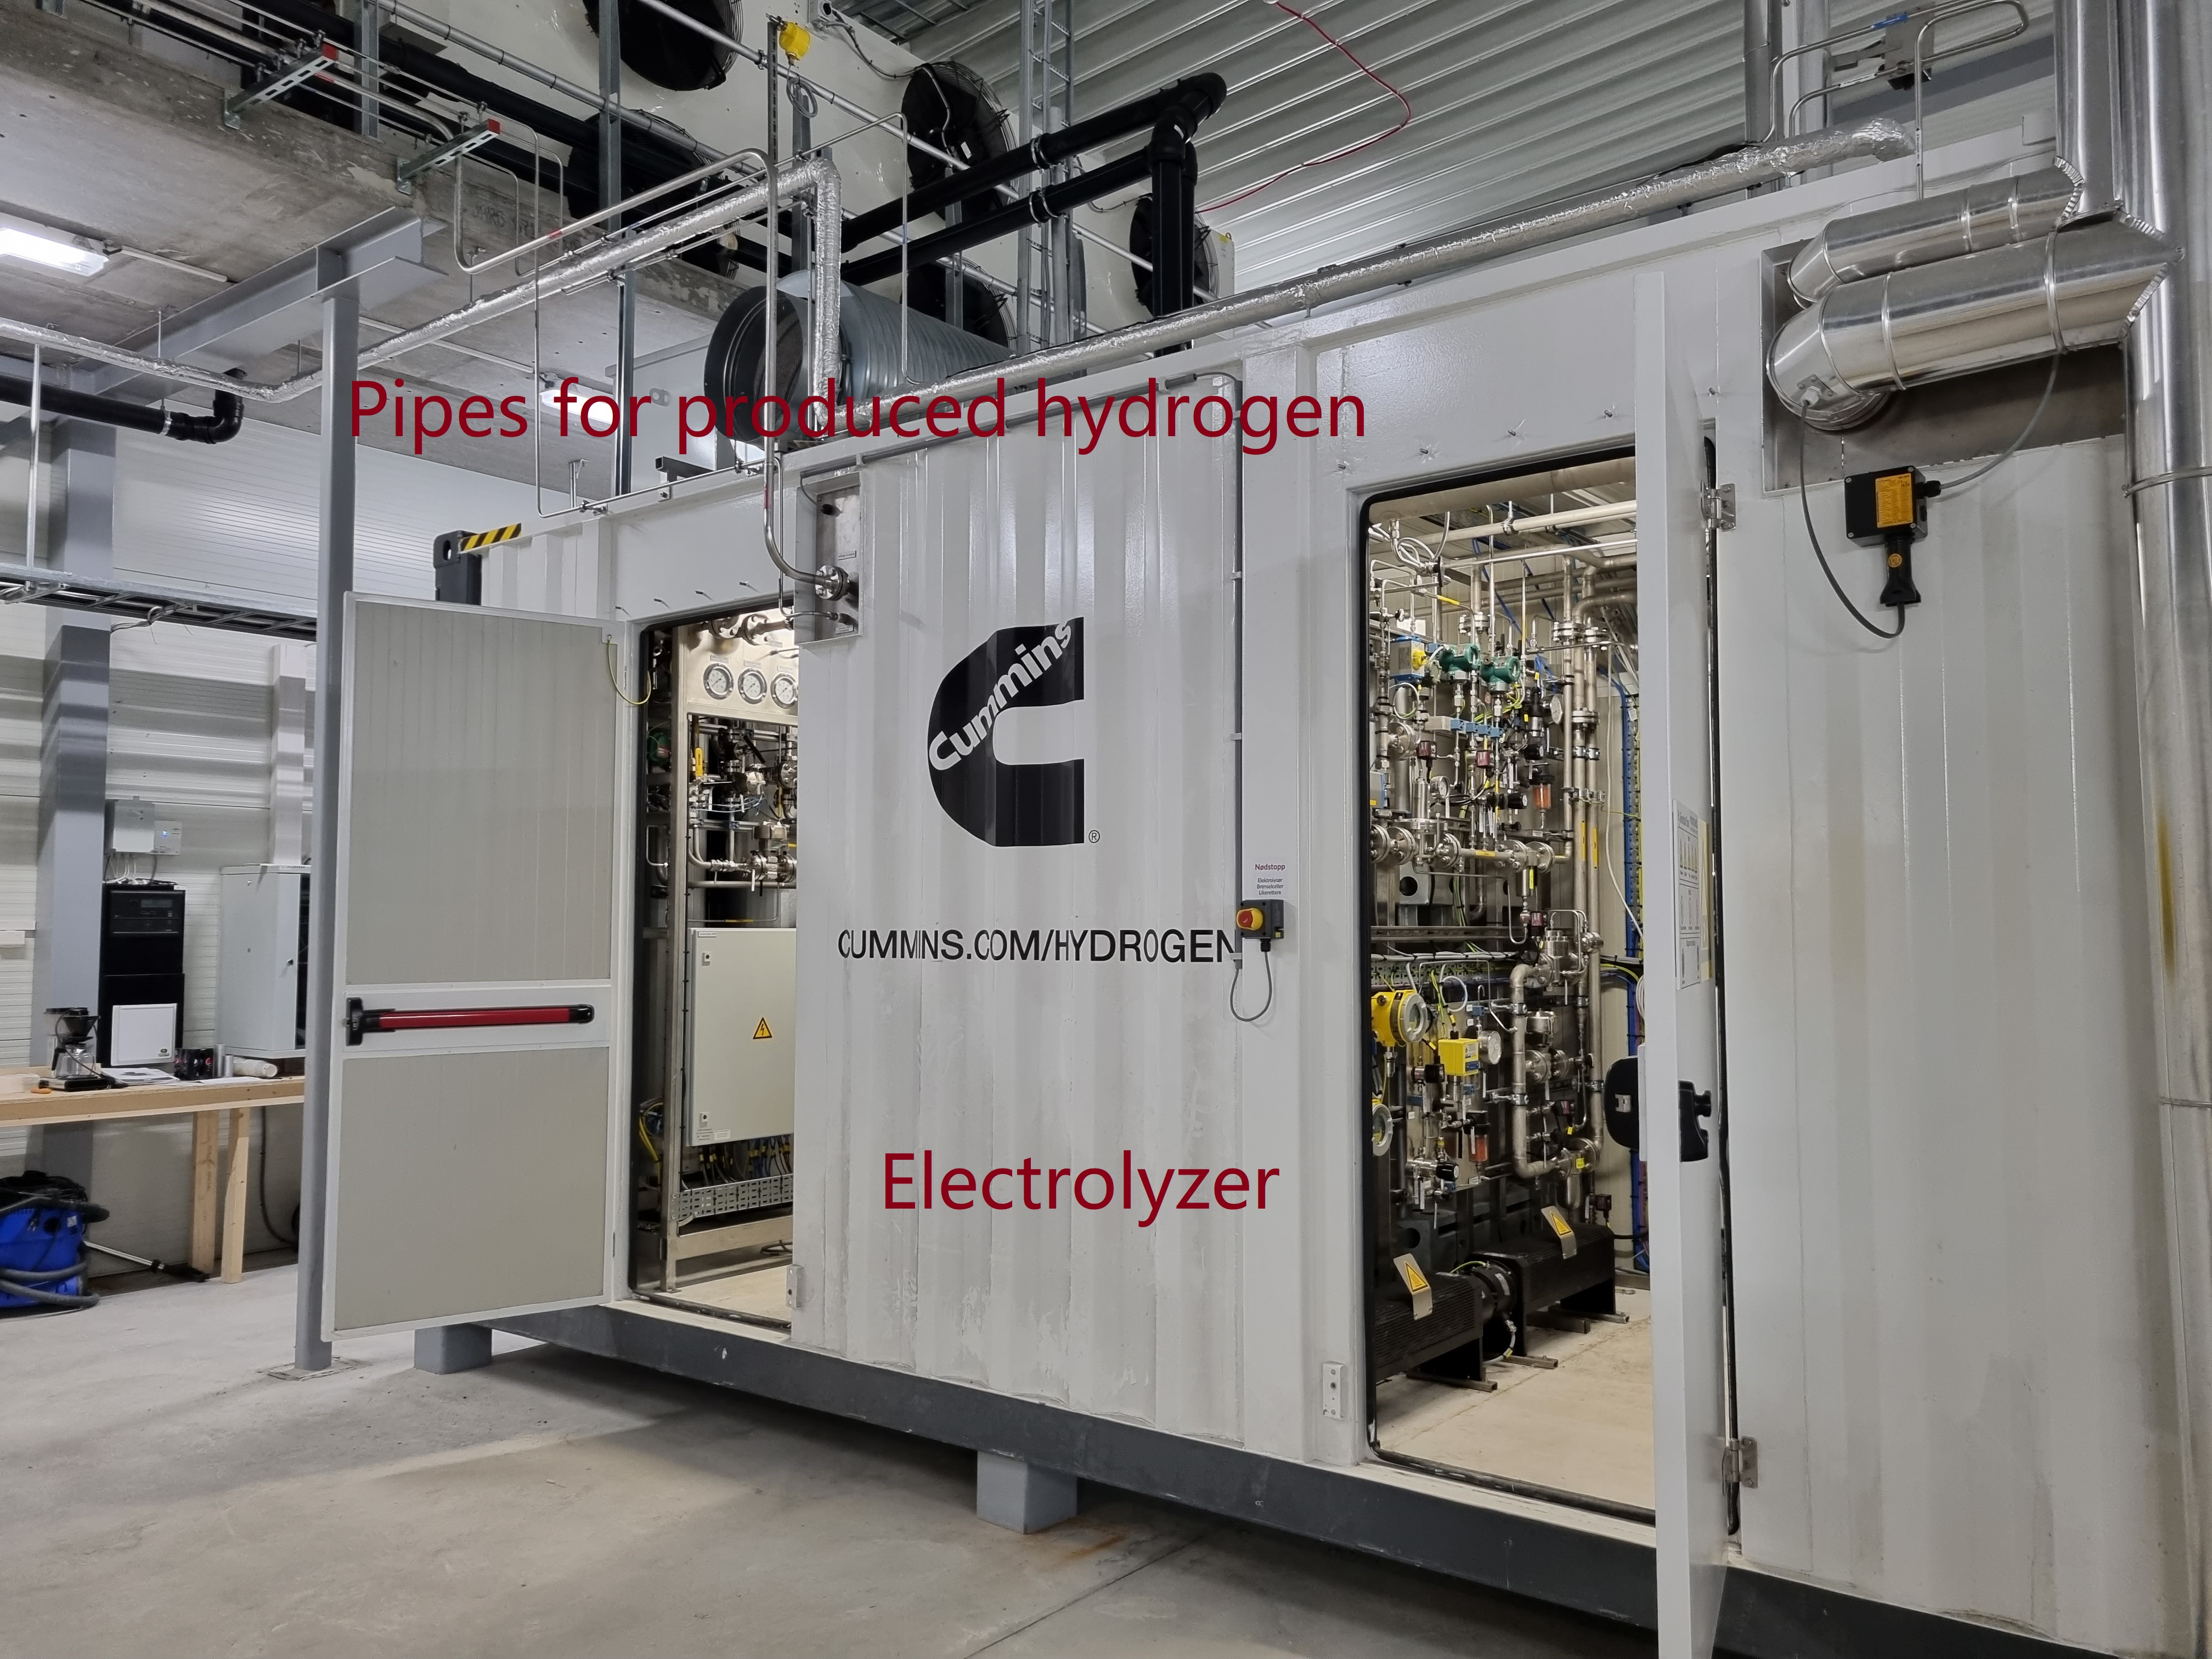
\includegraphics[scale=0.04]{container2}
\end{minipage}%
}

\frame{\frametitle{About the hydrogen plant}
\begin{minipage}{.5\textwidth}
\centering
\begin{enumerate}
\item Hydrogen is stored uncompressed in an outside tank
\item There are plans for expansion which include 700bar tanks and compressors
\item Unlike the tank, the containers need to be housed because of the extreme weather (winter) in Finnmark
\end{enumerate}
\end{minipage}%
\begin{minipage}{.5\textwidth}
\centering
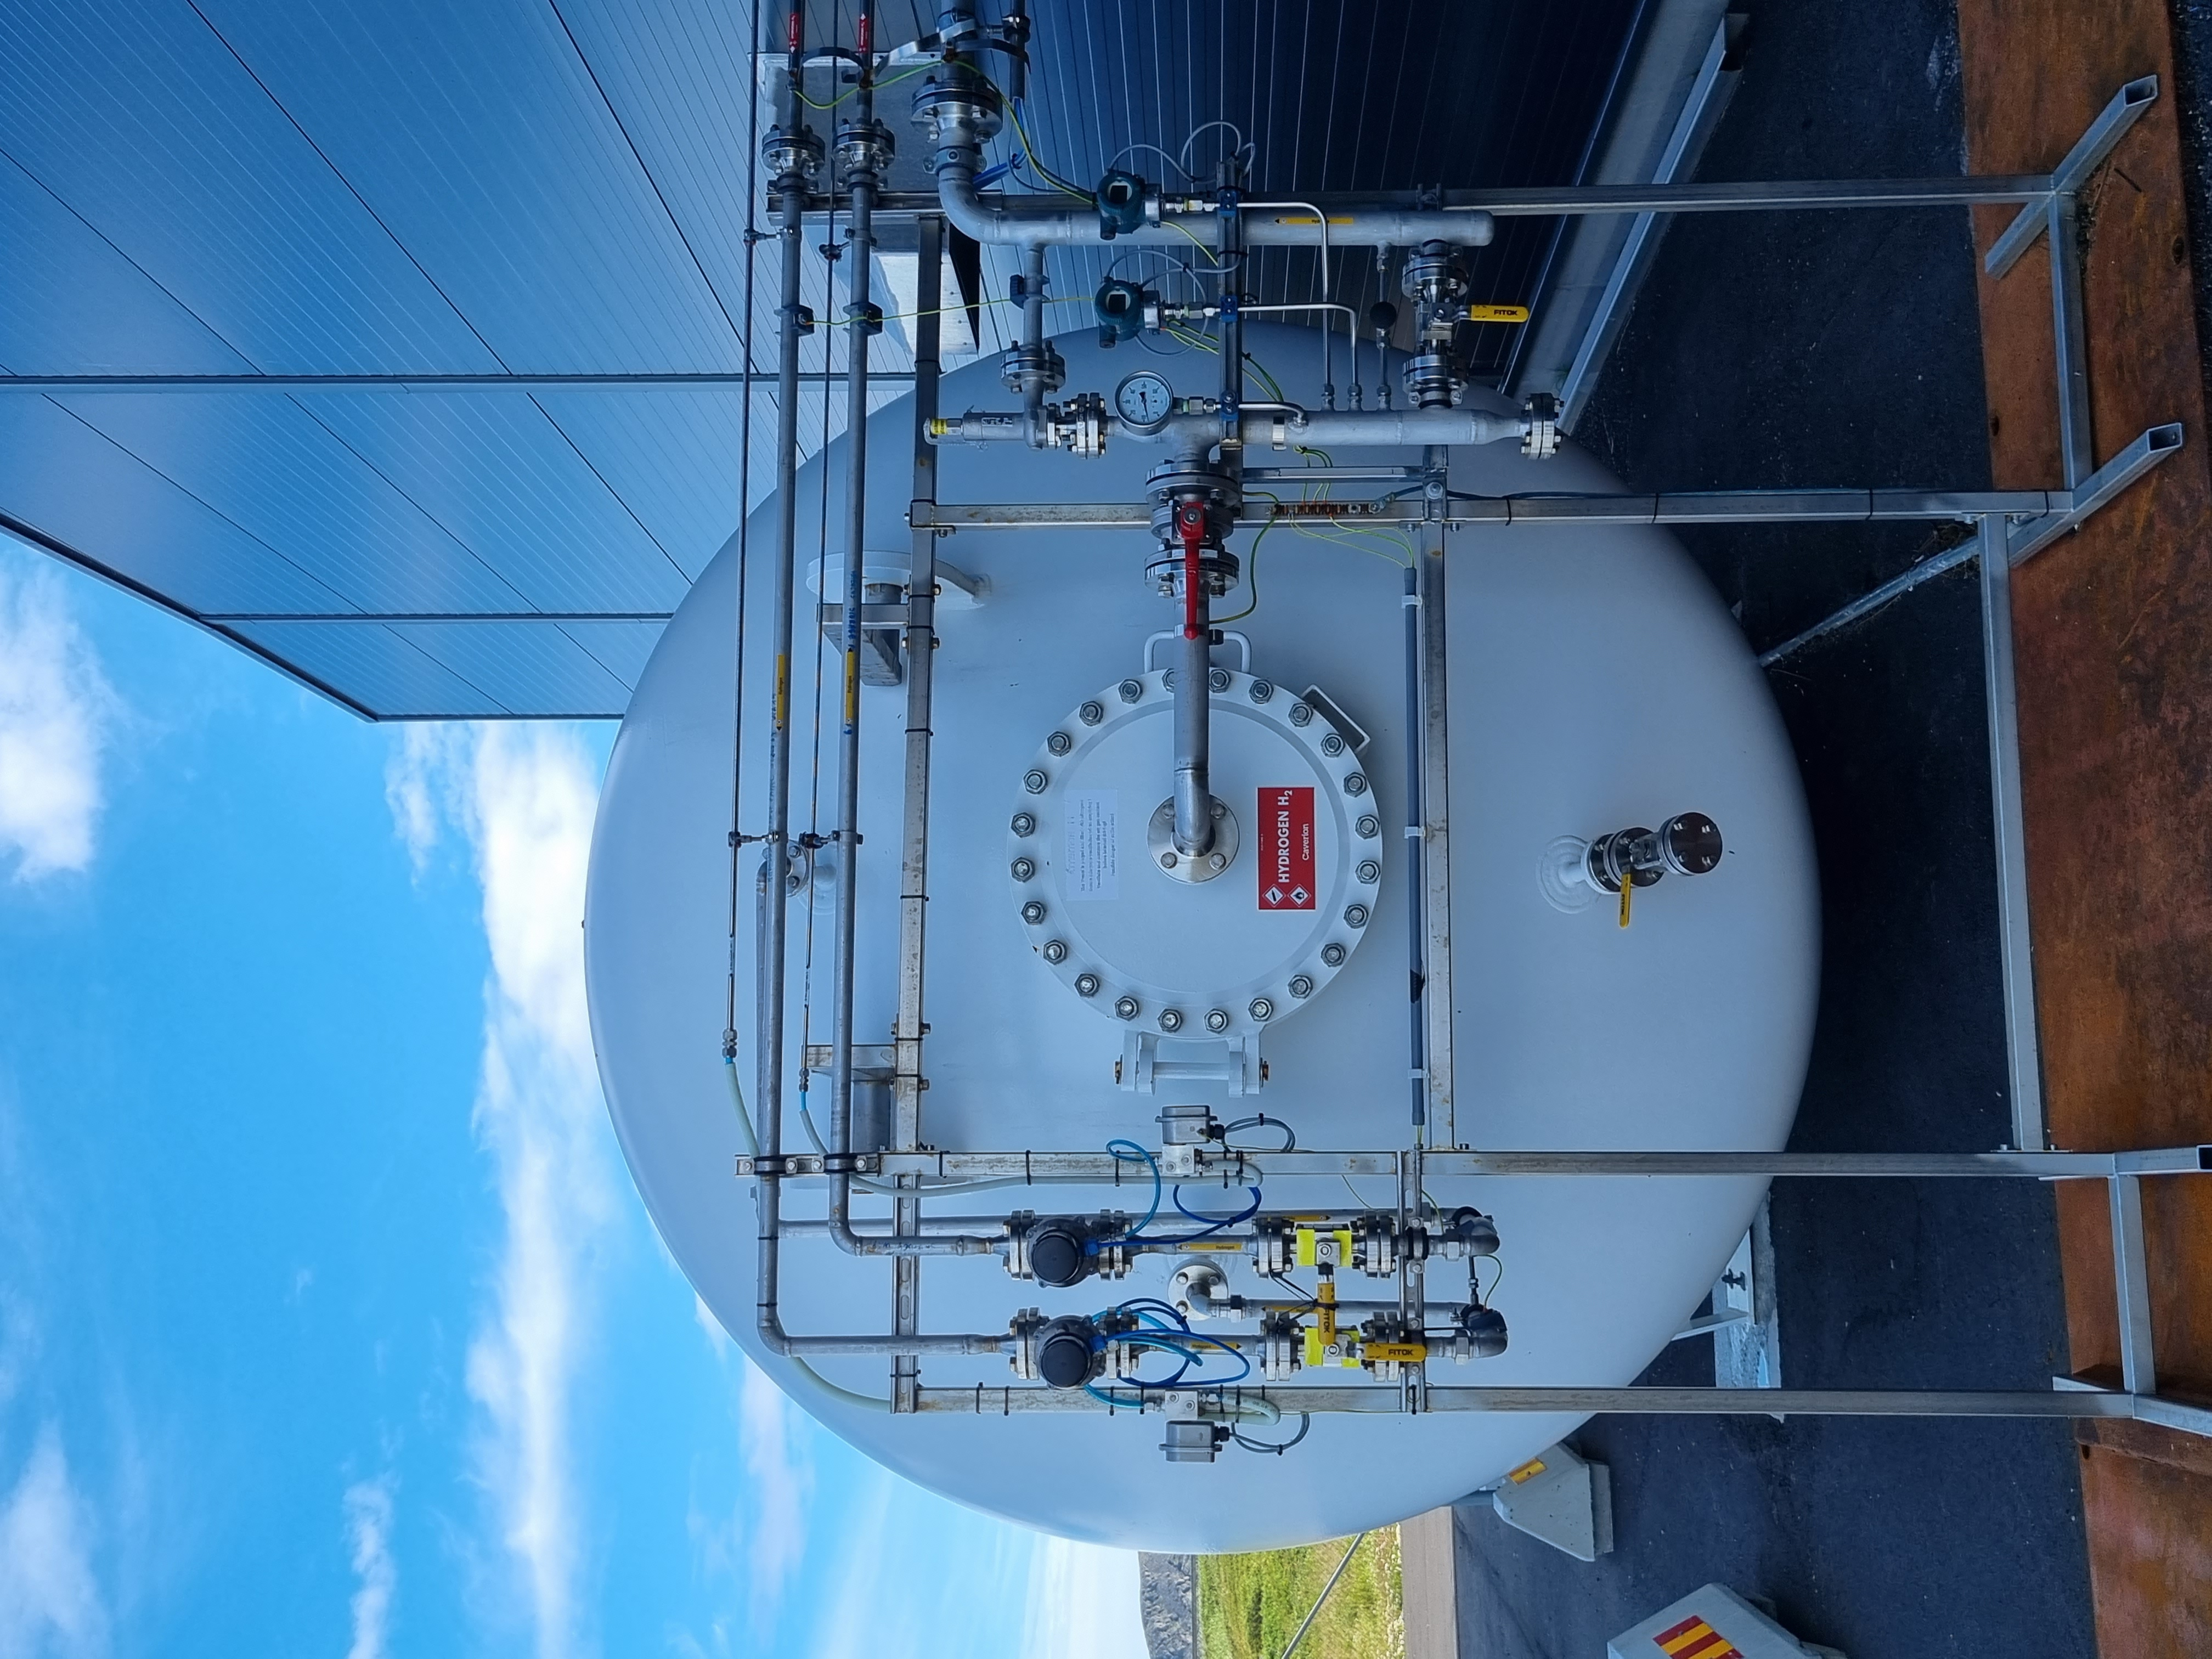
\includegraphics[scale=0.04, angle =270]{container3}
\end{minipage}%
}

\frame{\frametitle{Plans for expansion}
\centering
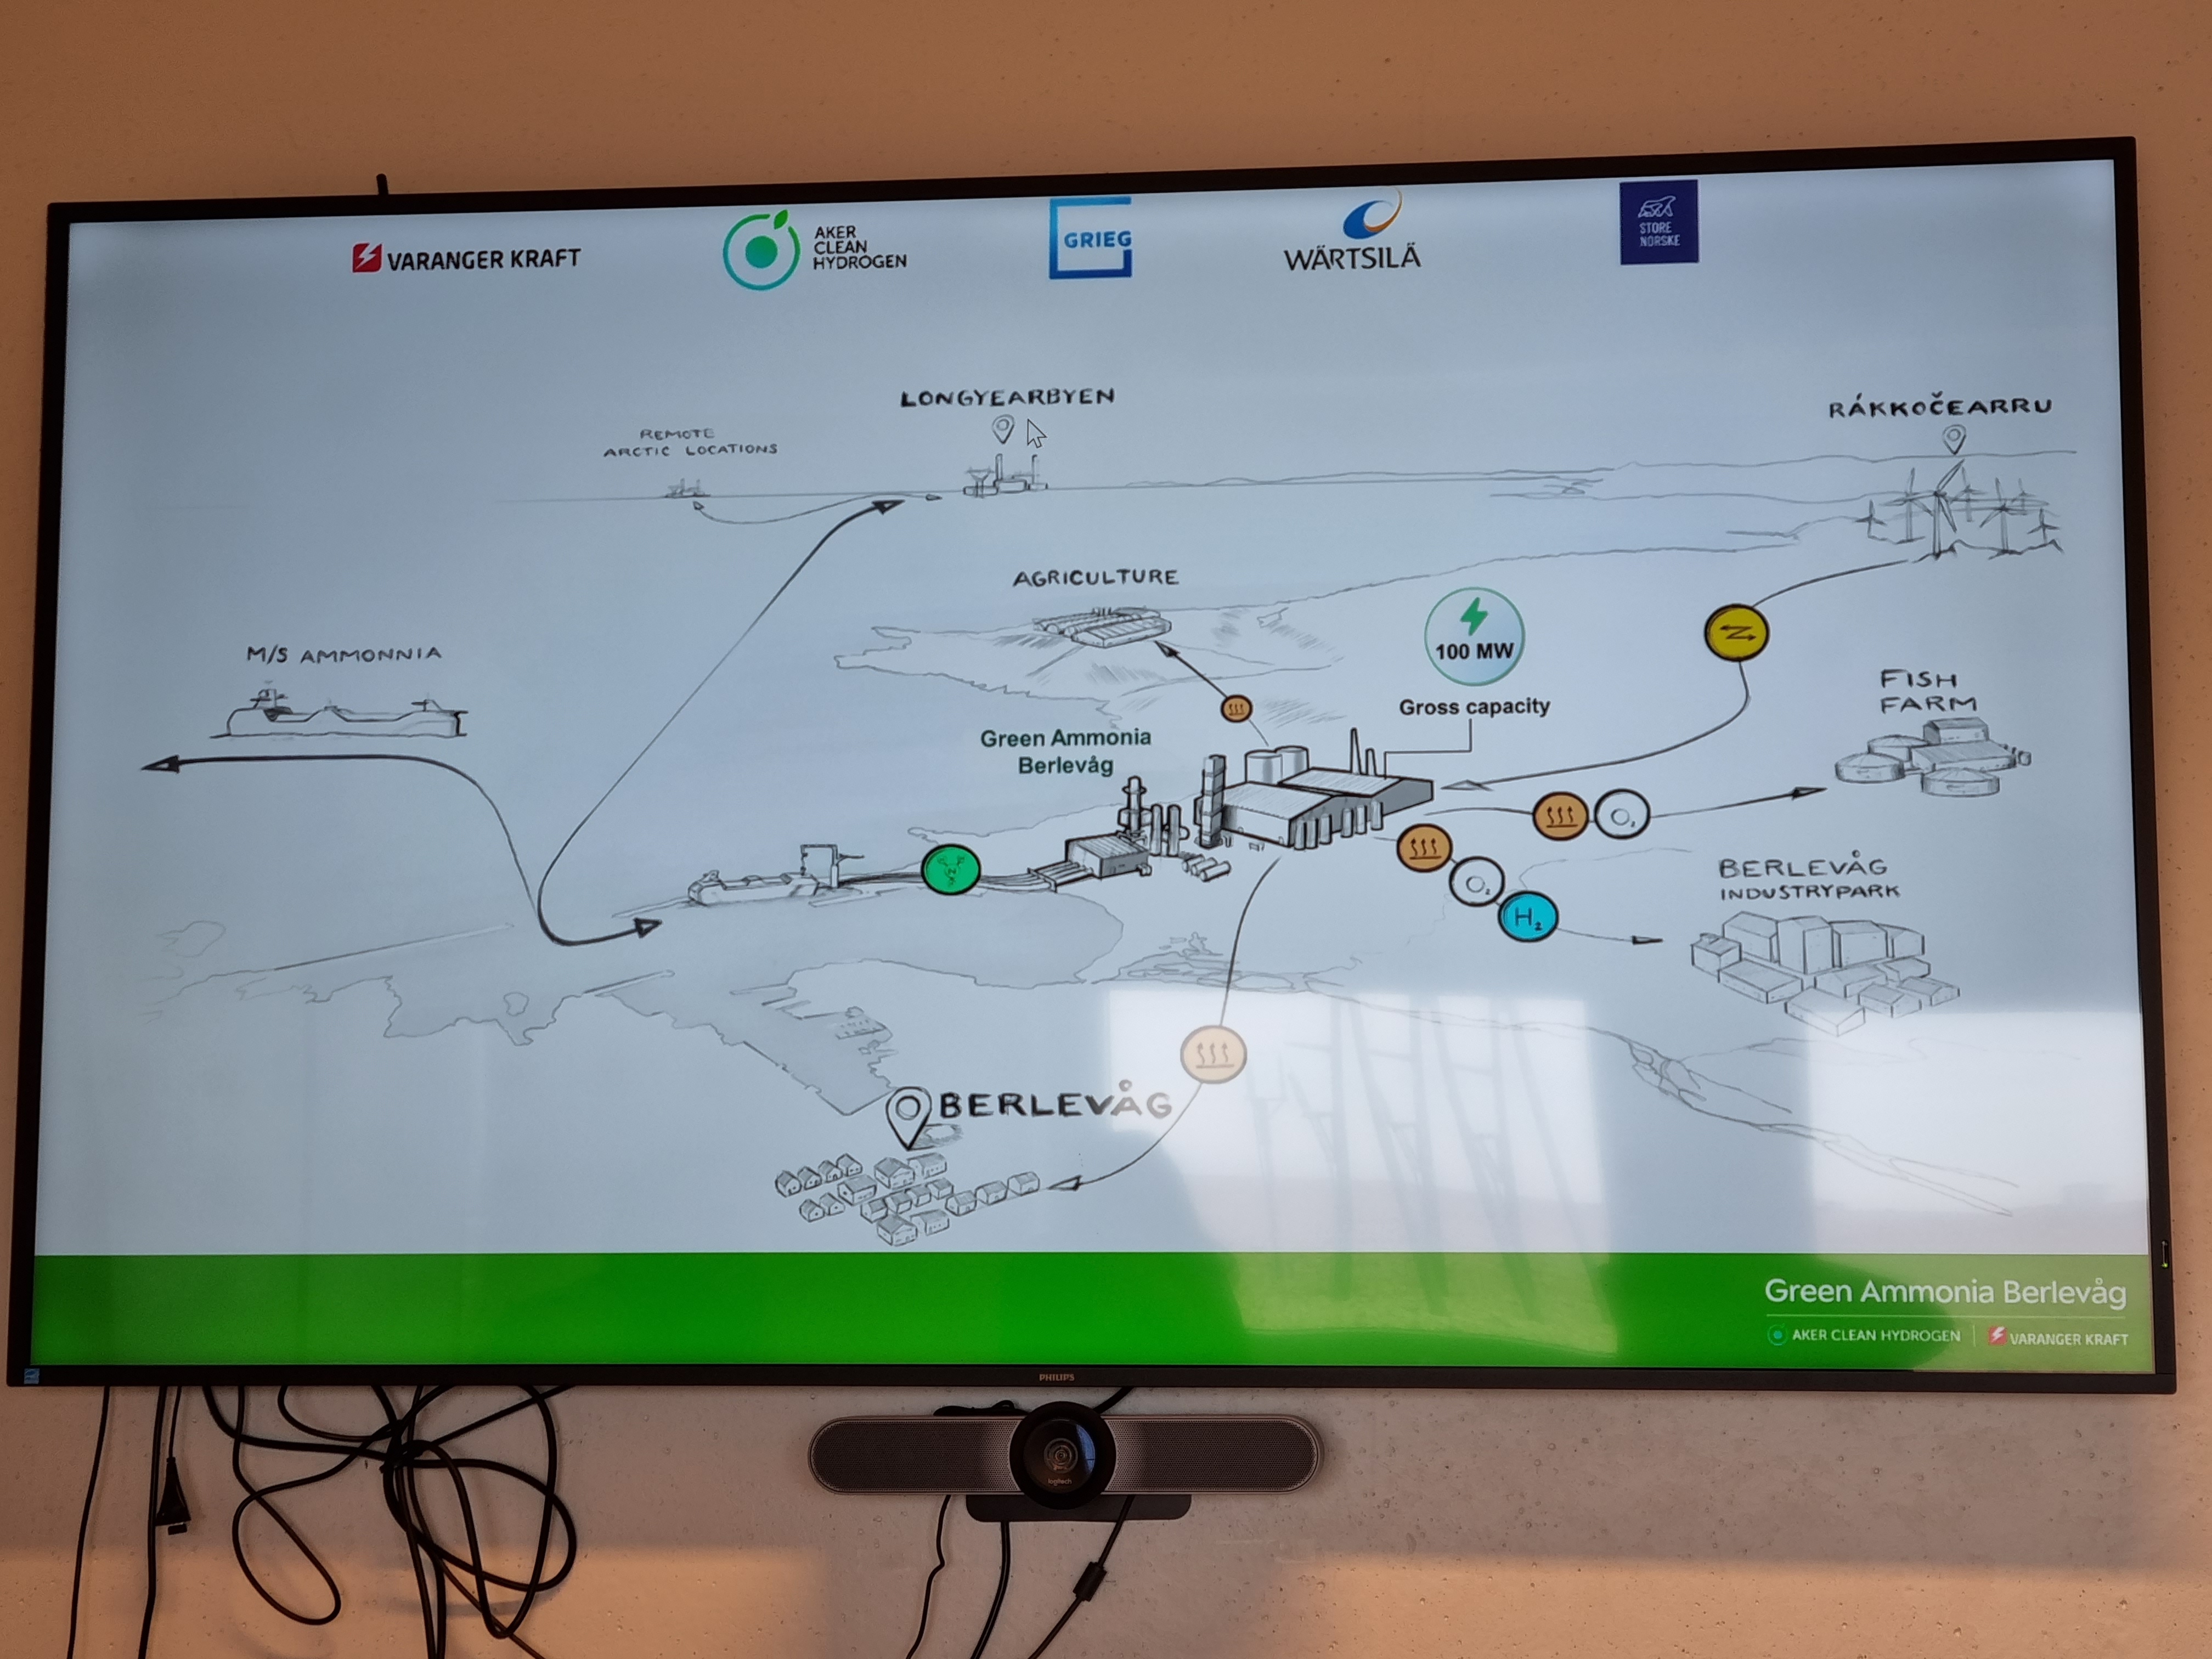
\includegraphics[scale=0.07]{i6}
}

\frame{\frametitle{Plans for expansion}
\begin{minipage}{.5\textwidth}
\centering
\begin{enumerate}
\item 100MW Ammonia plant next to the current hydrogen plant
\item Develop more use cases / consumers for the e-fuels
\item Eg. the Berlev\r{a}g region has many fishing industries, they and commercial shipping industries can be consumers for the e-fuels
\end{enumerate}
\end{minipage}%
\begin{minipage}{.5\textwidth}
\centering
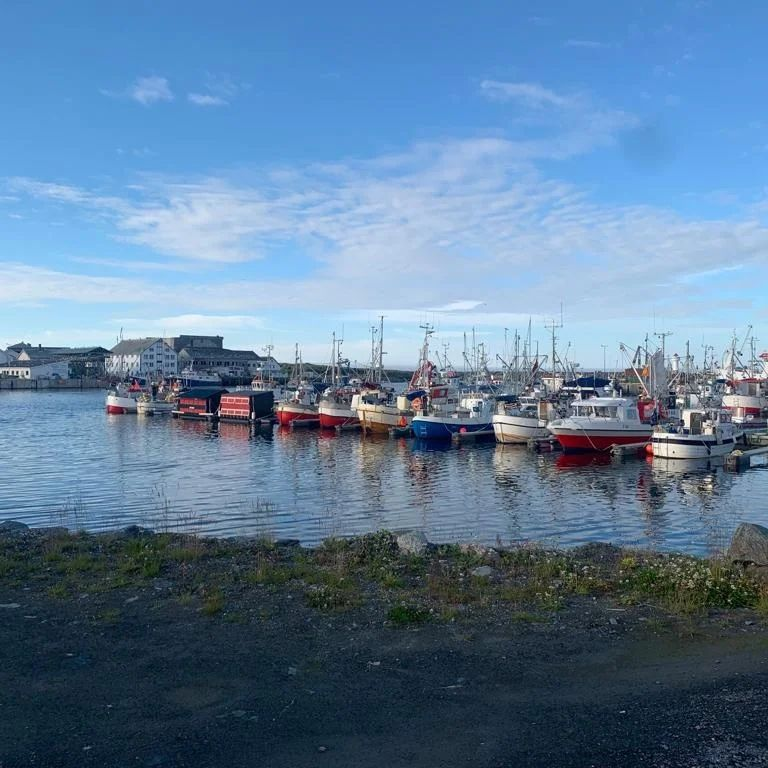
\includegraphics[scale=0.18]{i7}
\end{minipage}%
}

\frame{\frametitle{Additional challenges}
\begin{minipage}{.5\textwidth}
\centering
\begin{enumerate}
\item Indigenous people and their reindeers are disturbed by the wind park
\item Finnmark regions suffers from young people leaving to live in the south
\item Weather can be quite extreme (eg. there often is trouble with fog and air travel)
\end{enumerate}
\end{minipage}%
\begin{minipage}{.5\textwidth}
\centering
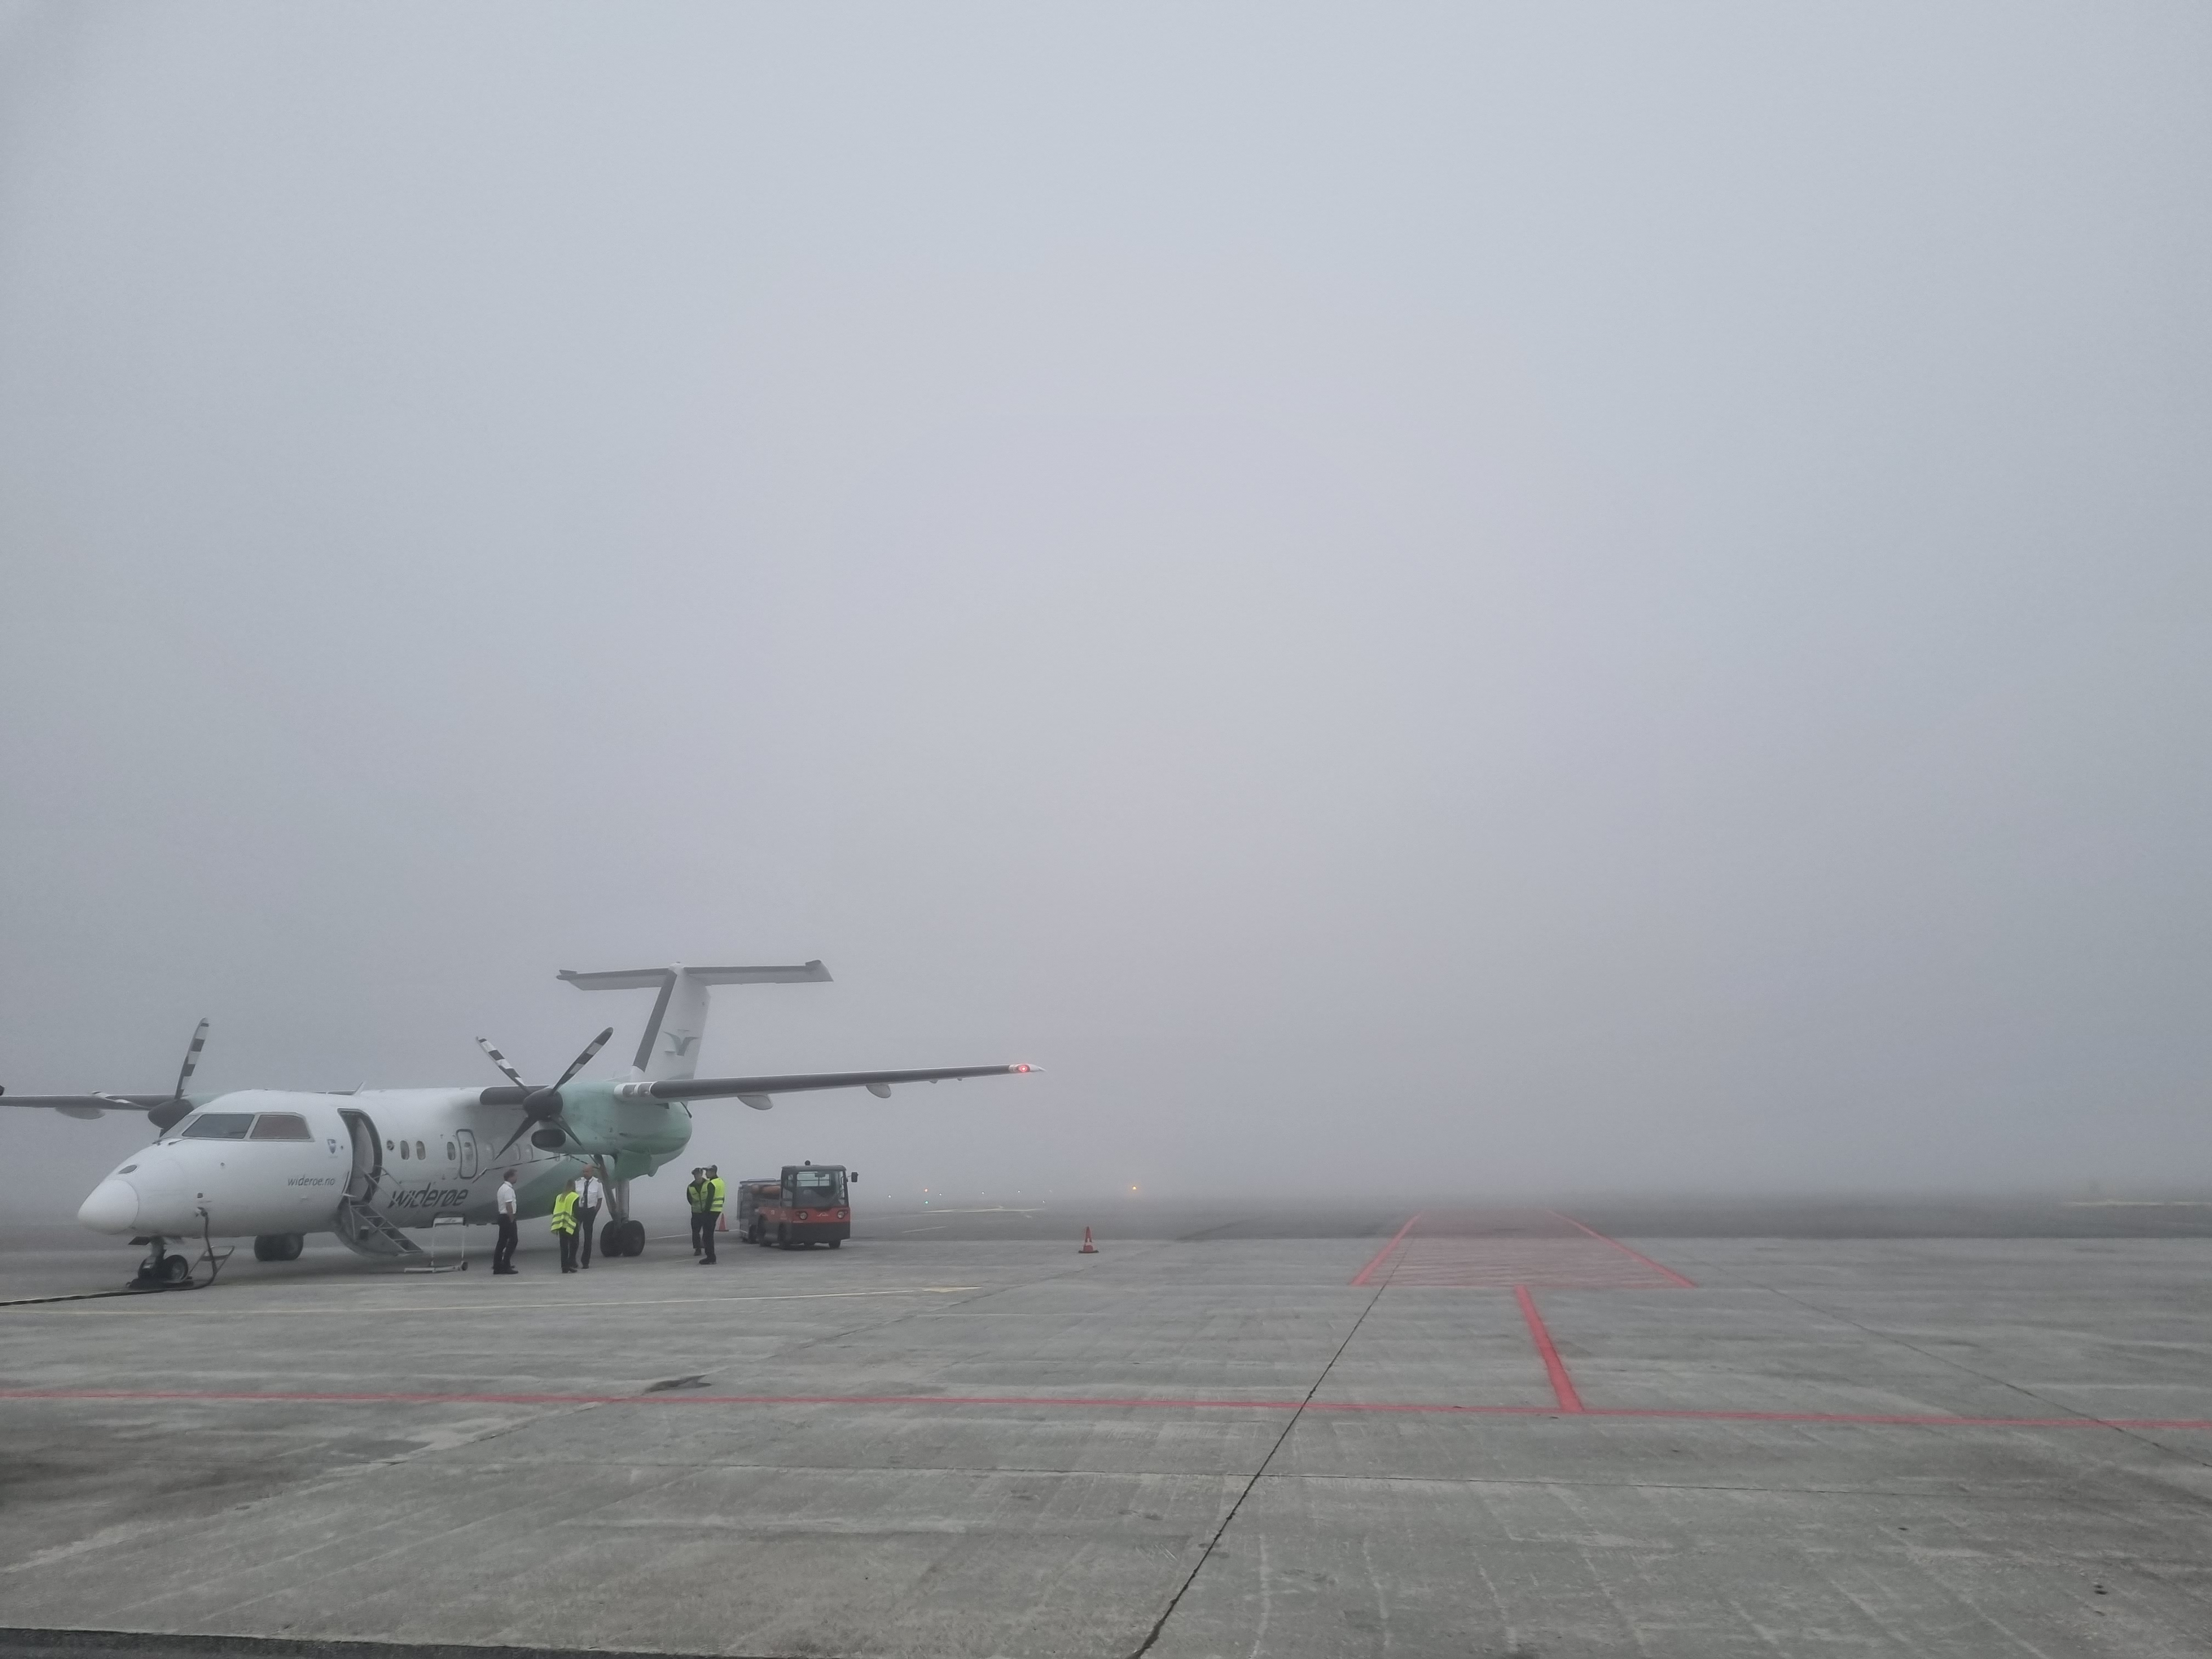
\includegraphics[scale=0.04]{i8}
\end{minipage}%
}

\frame{\frametitle{References}
\begin{enumerate}

\item \scriptsize Haeolus project website https://www.haeolus.eu/
\item  Varanger Kraft, https://www.varanger-kraft.no/hydrogen-1/
\item Cummins Hydrogen, https://www.cummins.com/new-power/technology/hydrogen-generation
\end{enumerate}
}

\end{document}